%Homework Template
%----------------------------------------
\documentclass[12pt]{article}
\usepackage[margin=1in]{geometry} 
\usepackage{amsmath,amsthm,amssymb,amsfonts}
\usepackage{ifthen}
\usepackage{pbox}
\usepackage{romannum}
\usepackage{centernot}
\usepackage{color,soul}
\usepackage{pgfplots}


\newenvironment{problem}[2][Problem]{\begin{trivlist}
\item[\hskip \labelsep {\bfseries #1}\hskip \labelsep {\bfseries #2.}]}{\end{trivlist}}
\renewcommand{\qedsymbol}{$\blacksquare$}
\usepackage{fancyhdr}
\usepackage{pst-plot}
\newcommand\ddfrac[2]{\frac{\displaystyle #1}{\displaystyle #2}}

%SetFonts
\pagestyle{fancy}
\rhead{Homework 2}
\lhead{Jugal Marfatia}
 
%----------------------------------------
% Assignment Title and Your Name
%----------------------------------------
\title{Homework 2}
\author{Jugal Marfatia \\ \\Microeconomics-1 \\ }
\date{September 6, 2017}
%----------------------------------------
\begin{document}
\maketitle

%========================================
%	START ANSWERS HERE
%========================================

\begin{problem}{1}. \\ \\
\textbf{a.}
\begin{flalign*} 
L& = \big[x_1^\rho + x_2^\rho \big]^{1/ \rho} + \lambda \big[w -p_1 x_1 - p_2 x_2 \big]& \\ \\
\text{F.O.C's are below: }
\\
\\
\frac{dL}{dx_1} & = x_1^{\rho - 1 } \big[x_1^\rho + x_2^\rho \big]^{\frac{1-\rho}{\rho}} - \lambda p_1 = 0& (1)& \\ \\
\frac{dL}{dx_2} & = x_2^{\rho - 1 } \big[x_1^\rho + x_2^\rho \big]^{\frac{1-\rho}{\rho}} - \lambda p_2 = 0& (2)& \\ \\
\frac{dL}{d\lambda} & = w -p_1 x_1 - p_2 x_2 = 0& (3)& \\ \\
\end{flalign*} 
Dividing equation 1 and 2 we get: 
\\
\\
$\ddfrac{x_1^{\rho - 1 } \big[x_1^\rho + x_2^\rho \big]^{\frac{1-\rho}{\rho}}}{x_2^{\rho - 1 } \big[x_1^\rho + x_2^\rho \big]^{\frac{1-\rho}{\rho}}} = \ddfrac{\lambda p_1}{\lambda p_2} \iff \ddfrac{x_1^{\rho - 1 }}{x_2^{\rho - 1 }} = \ddfrac{p_1}{ p_2} \iff x_1 = x_2 \bigg(\ddfrac{p_1}{ p_2}\bigg)^{\frac{1}{\rho-1}} $
\\
\\
\\
Next plugging $x_1 $ back into the budget constraint we get:
\\
\\
$p_1 x_2 \bigg(\ddfrac{p_1}{ p_2}\bigg)^{\frac{1}{\rho-1}} + p_2 x_2 = w \iff x_2^* = \ddfrac{w}{p_1  \bigg(\ddfrac{p_1}{ p_2}\bigg)^{\frac{1}{\rho-1}} + p_2}$\hspace{10mm}  (Walrasian demand for $x_2$)
\\
\\Further using symmetry we get:
\\
\\
$x_1^* = \ddfrac{w}{p_2  \bigg(\ddfrac{p_2}{ p_1}\bigg)^{\frac{1}{\rho-1}} + p_1}$ \hspace{10mm} (Walrasian demand for $x_1$)
\\
\\
\\
\textbf{b.} When $\rho \rightarrow 0 $.
\\
\\
$x_1^* = \ddfrac{w}{p_2  \bigg(\ddfrac{p_1}{ p_2}\bigg) + p_1}= \ddfrac{w}{2 p_1}$ \hspace{18mm} $x_2^* = \ddfrac{w}{p_1  \bigg(\ddfrac{p_2}{ p_1}\bigg) + p_2}= \ddfrac{w}{2 p_2}$ 
\\
\\
\end{problem}
\begin{problem}{2}. \\ \\
\textbf{a.}
\begin{flalign*} 
p \cdot x & = \Bigg[ \frac{p_1}{p_1} \bigg(a_1 + b_1 w + \sum_{j=1}^{k}\gamma_{1j} p_j \bigg) +\frac{p_2}{p_2} \bigg(a_2 + b_2 w + \sum_{j=i}^{k}\gamma_{2j} p_j \bigg)+ .... +\frac{p_k}{p_k} \bigg(a_k + b_k w + \sum_{j=i}^{k}\gamma_{kj} p_j \bigg)  \Bigg] & \\ \\
& = \Bigg[  \bigg(a_1 + b_1 w + \sum_{j=i}^{k}\gamma_{1j} p_j \bigg) +\bigg(a_2 + b_2 w + \sum_{j=i}^{k}\gamma_{2j} p_j \bigg)+ .... + \bigg(a_k + b_k w + \sum_{j=1}^{k}\gamma_{kj} p_j \bigg)  \Bigg] & \\ \\
& = \Bigg[  \sum_{i=1}^{k}a_i + w \sum_{i=1}^{k} b_i  + \sum_{i=1}^{k} \sum_{j=1}^{k}\gamma_{ij} p_j  \Bigg] & \\
\end{flalign*} 
Therefore when $ \sum_{i=1}^{k}a_i = 0,\text{ } \sum_{i=1}^{k} b_i = 1 \text{ } \& \text{ } \sum_{i=1}^{k} \sum_{j=1}^{k}\gamma_{ij} p_j = 0 $ the walras law is satisfied. 
\\ \\
\\
\textbf{b.}
\begin{flalign*} 
p \cdot x & = \Bigg[ \frac{w p_1}{p_1} \bigg(a_1 + b_1 log(w) + \sum_{j=1}^{k}\gamma_{1j} log(p_j) \bigg) +....+\frac{w p_k}{p_k} \bigg(a_k + b_k log(w) + \sum_{j=i}^{k}\gamma_{kj} log(p_j) \bigg)  \Bigg] & \\ \\
& = w \Bigg[  \bigg(a_1 + b_1 log (w) + \sum_{j=i}^{k}\gamma_{1j} log(p_j) \bigg) + .... + \bigg(a_k + b_k log(w) + \sum_{j=1}^{k}\gamma_{kj} log(p_j) \bigg)  \Bigg] & \\ \\
& = w \Bigg[  \sum_{i=1}^{k}a_i + log(w) \sum_{i=1}^{k} b_i  + \sum_{i=1}^{k} \sum_{j=1}^{k}\gamma_{ij} log(p_j)  \Bigg] & \\
\end{flalign*} 
Therefore the walras law is satisfied under 2 conditions. 
\\
\\
Condition 1 when,  $ \sum_{i=1}^{k}a_i = 0,\text{ } \sum_{i=1}^{k} b_i = \frac{1}{log(w)} \text{ } \& \text{ } \sum_{i=1}^{k} \sum_{j=1}^{k}\gamma_{ij} p_j = 0 $ 
\\ \\
Condition 2 when,  $ \sum_{i=1}^{k}a_i = 1,\text{ } \sum_{i=1}^{k} b_i = 0 \text{ } \& \text{ } \sum_{i=1}^{k} \sum_{j=1}^{k}\gamma_{ij} p_j = 0 $ 
\\
\\
\\
\textbf{c.}
\begin{flalign*} 
p \cdot x & = \Bigg[ \frac{p_1}{p_1} \bigg(a_1 + b_1 w + \gamma_1 w^2 \bigg) +....+\frac{p_k}{p_k} \bigg(a_k + b_k w + \sum_{j=i}^{k}\gamma_{k} w2 \bigg)  \Bigg] & \\ \\
& =  \Bigg[  \bigg(a_1 + b_1 w + \gamma_{1} log(p_j) \bigg) + .... + \bigg(a_k + b_k w + \gamma_{k} w^2 \bigg)  \Bigg] & \\ \\
& =  \Bigg[  \sum_{i=1}^{k}a_i + w \sum_{i=1}^{k} b_i  + w^2 \sum_{i=1}^{k} \gamma_{i}  \Bigg] & \\
\end{flalign*} 
Therefore the walras law is satisfied under 2 conditions. 
\\
\\
Condition 1, when $ \sum_{i=1}^{k}a_i = 0,\text{ } \sum_{i=1}^{k} b_i = 0 \text{ } \& \text{ } \sum_{i=1}^{k} \gamma_{i}  = \frac{1}{w}  $ the walras law is satisfied.
\\
\\
Condition 2, when $ \sum_{i=1}^{k}a_i = 0,\text{ } \sum_{i=1}^{k} b_i = 1 \text{ } \& \text{ } \sum_{i=1}^{k} \gamma_{i}  = 0  $ the walras law is satisfied.
\\
\\
\end{problem}
\pagebreak
\begin{problem}{3}. \\ \\ 
\textbf{a.} Random Demand. In the case of random demand the person can end up choosing a bundle $x(p'w') $ given $B_{p',w'} $ which was affordable under the the old $ B_{p,w} $ (As shown in the below figure). In other terms, in this case $ p\cdot x(p',w') \leq w $ and $x(p',w') \neq x(p,w) $ however$,  p' \cdot x(p,w) < w'$ which violates WARP. 
\\
\\
\\
\begin{tikzpicture}
\begin{axis}[
    axis lines = left,
    xlabel = $x_1 $,
    ylabel = {$x_2$},
    yticklabels={,,},
    xticklabels={,,}
]
%Below the red parabola is defined
\addplot [
	dashed,
    domain=-0:120, 
    samples=100, 
    color=red,
]
{60 - 0.5*x};
\addlegendentry{$B_{p, w}$}
%Here the blue parabloa is defined
\addplot [
    domain=-0:200, 
    samples=100, 
    color=blue,
    ]
    {40 - 0.2*x};
\addlegendentry{$B_{p', w'}$}
\end{axis}
\foreach \Point/\PointLabel in {(1,3.2)/{x(p',w')}, (3,1.55)/{x(p,w)}}
    \draw[fill=black] \Point circle (0.1) node[below] {$\PointLabel$};
\end{tikzpicture}
\\
\\
\textbf{b.} Average Demand. In the case of average demand the bundle selected will always be at the intersection of any two arbitrary budget constraint. i.e. the bundle will be affordable under both budget constraint and the same bundle will be chosen under both budget constraint. Thus we have,
\\
$p'  \cdot x(p, w) \leq w' $ and $ p \cdot x(p', w') \leq w \implies x(p',w') = x(p,w). $, which implies that WARP is satisfied. 
\\
\\
\begin{tikzpicture}
\begin{axis}[
    axis lines = left,
    xlabel = $x_1 $,
    ylabel = {$x_2$},
    yticklabels={,,},
    xticklabels={,,}
]
%Below the red parabola is defined
\addplot [
	dashed,
    domain=-0:120, 
    samples=100, 
    color=red,
]
{60 - 0.5*x};
\addlegendentry{$B_{p, w}$}
%Here the blue parabloa is defined
\addplot [
    domain=-0:200, 
    samples=100, 
    color=blue,
    ]
    {40 - 0.2*x};
\addlegendentry{$B_{p', w'}$}
\end{axis}
\foreach \Point/\PointLabel in {(2.2,2.55)/{$x(p',w') = x(p,w) $}}
    \draw[fill=black] \Point circle (0.1) node[above right] {$\PointLabel$};
\end{tikzpicture}
\\
\\
\textbf{c.} Conspicuous demand. In the conspicuous demand case we would end up at the end points of the budget constraint (As shown below). And thus in this case, the person can end up choosing a bundle $x(p'w') $ given $B_{p',w'} $ which was affordable under the the old $ B_{p,w} $. In other terms, in this case $ p\cdot x(p',w') \leq w $ and $x(p',w') \neq x(p,w) $ however$,  p' \cdot x(p,w) < w'$ which violates WARP. 
\\
\\
\begin{tikzpicture}
\begin{axis}[
    axis lines = left,
    xlabel = $x_1 $,
    ylabel = {$x_2$},
    yticklabels={,,},
    xticklabels={,,}
]
%Below the red parabola is defined
\addplot [
	dashed,
    domain=-0:120, 
    samples=100, 
    color=red,
]
{60 - 0.5*x};
\addlegendentry{$B_{p, w}$}
%Here the blue parabloa is defined
\addplot [
    domain=-0:200, 
    samples=100, 
    color=blue,
    ]
    {40 - 0.2*x};
\addlegendentry{$B_{p', w'}$}
\end{axis}
\foreach \Point/\PointLabel in {(0,3.8)/{x(p',w')}, (4,0)/{x(p,w)}}
    \draw[fill=black] \Point circle (0.1) node[above left] {$\PointLabel$};
\end{tikzpicture}
\\
\\
\end{problem}
\begin{problem}{4}. \\ \\ 
\textbf{a.}
\\
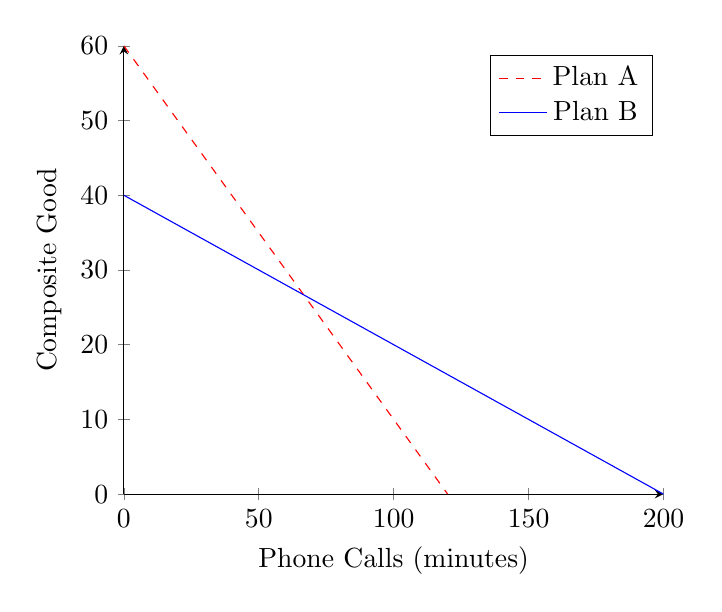
\begin{tikzpicture}
\begin{axis}[
    axis lines = left,
    xlabel = Phone Calls (minutes),
    ylabel = {Composite Good},
]
%Below the red parabola is defined
\addplot [
	dashed,
    domain=-0:120, 
    samples=100, 
    color=red,
]
{60 - 0.5*x};
\addlegendentry{Plan A}
%Here the blue parabloa is defined
\addplot [
    domain=-0:200, 
    samples=100, 
    color=blue,
    ]
    {40 - 0.2*x};
\addlegendentry{Plan B}
 
\end{axis}
\end{tikzpicture}
 \\ \\ 
\textbf{b.} As shown below the line segment from point A to point B represents the set of baskets Jeremy may purchase if his behavior is consistent with WARP. 
\\
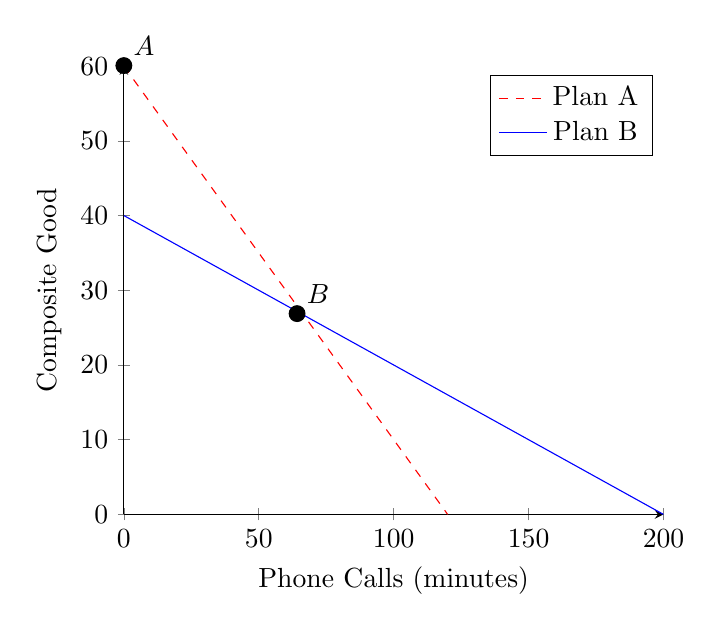
\begin{tikzpicture}
\begin{axis}[
    axis lines = left,
    xlabel = Phone Calls (minutes),
    ylabel = {Composite Good},
]
%Below the red parabola is defined
\addplot [
	dashed,
    domain=-0:120, 
    samples=100, 
    color=red,
]
{60 - 0.5*x};
\addlegendentry{Plan A}
%Here the blue parabloa is defined
\addplot [
    domain=-0:200, 
    samples=100, 
    color=blue,
    ]
    {40 - 0.2*x};
\addlegendentry{Plan B}
\end{axis}
\foreach \Point/\PointLabel in {(0,5.7)/A, (2.2,2.55)/B}
    \draw[fill=black] \Point circle (0.1) node[above right] {$\PointLabel$};
\end{tikzpicture}
\end{problem}
\begin{problem}{5}. \\ \\ 
\textbf{a.} No in that case the preferences are not convex because the budget set consists of only two point. In other words any combination of the two points is not possible.
\\
\\
\textbf{b.} Let $x, y \in B_{p,w} $. \\
\\
Therefore $ \forall a \in [0,1],  a x + (1- a) y \leq  a w + (1- a) w = w \implies a x + (1- a) y \leq w \implies a x + (1- a) y \in B_{p,w} \implies B_{p,w}$ is convex as well. 
\\
\\
\end{problem}
\begin{problem}{6}. \\ \\ Definition 2.F.1 states: \\
\\
If  $ p \cdot x(p', w') \leq w$ and $x(p',w') \neq x(p,w) \implies p'  \cdot x(p, w) > w'    $
\\
\\
Which is equivalent to $ p'  \cdot x(p, w) \leq w' \implies p \cdot x(p', w') > w$ or $x(p',w') = x(p,w).$
\\
\\
Therefore if $p'  \cdot x(p, w) \leq w' $ and $ p \cdot x(p', w') \leq w \implies x(p',w') = x(p,w). $ In other words if two bundles are affordable under two budget sets, then the bundle chosen under one budget set is equal to the bundle chosen under the other budget. 
\\
\\
Putting this in the context of choice structure we get \\
\\
$ \forall B, B' \in \beta  $ if $ C(B) \subset B'  $ and $ C(B') \subset B \implies C(B) = C(B')$
\\
\\
Which is equivalent to:
\\
\\
$ \forall B, B' \subset \beta $ if $ x, y \in B$, $ x, y \in B'  $, $ x \in C(B) $ and $ y \in C(B') \implies x \in C(B'). $ (1.C.1)
\\
\\
Therefore, for the Walrasian demand functions, the definition of the weak axiom given in Definition 2.F.1 coincides with that in Definition 1.C.1.

\end{problem}
\end{document}
